\documentclass[12pt]{article} 

\usepackage{fullpage}
\usepackage{bookmark}
\usepackage{amsmath}
\usepackage{amssymb}
\usepackage[dvipsnames]{xcolor}
\usepackage{hyperref} % for the URL
\usepackage[shortlabels]{enumitem}
\usepackage{mathtools}
\usepackage[most]{tcolorbox}
\usepackage[amsmath,standard,thmmarks]{ntheorem} 
\usepackage{physics}
\usepackage{pst-tree} % for the trees
\usepackage{verbatim} % for comments, for version control
\usepackage{tabu}
\usepackage{tikz}
\usepackage{float}
\usepackage{siunitx}
\usepackage{physunits}
\usepackage{pgfplots}

% From the Plot video

\usepackage[LGR,T1]{fontenc}
\usepackage[utf8]{inputenc}
\usepackage{lmodern}
\usepackage{microtype}
\usepackage{upgreek}
\usepackage[misc]{ifsym}

\usepackage{pgfplots}
	\usetikzlibrary{
		calc,
		patterns,
		positioning
	}
	\pgfplotsset{
		compat=1.16,
		samples=200,
		clip=false,
		my axis style/.style={
			axis x line=middle,
			axis y line=middle,
			legend pos=outer north east,
			axis line style={
				->,
			},
			legend style={
				font=\footnotesize
			},
			label style={
				font=\footnotesize
			},
			tick label style={
				font=\footnotesize
			},
			xlabel style={
				at={
					(ticklabel* cs:1)
				},
				anchor=west,
				font=\footnotesize,
			},
			ylabel style={
				at={
					(ticklabel* cs:1)
				},
				anchor=west,
				font=\footnotesize,
			},
			xlabel=$t$,
			ylabel=$\vec v (\m \tx{[East]})$
		},
	}
	\tikzset{
		>=stealth
	}


    \pgfplotsset{my style/.append style={axis x line=middle, axis y line=
           middle, xlabel={$t$}, axis equal }}

%%% Tables and figures packages

\usepackage{float}
\usepackage{caption}
	\captionsetup{
		format=plain,
		labelfont=bf,
		font=small,
		justification=centering
	}
	
%%% Numbers and sets

\newcommand{\E}{\mathrm{e}}
\newcommand{\tx}[1]{\text{#1}}


% floor, ceiling, set
\DeclarePairedDelimiter{\ceil}{\lceil}{\rceil}
\DeclarePairedDelimiter{\floor}{\lfloor}{\rfloor}
\DeclarePairedDelimiter{\set}{\lbrace}{\rbrace}
\DeclarePairedDelimiter{\iprod}{\langle}{\rangle}

\DeclareMathOperator{\Int}{int}
\DeclareMathOperator{\mean}{mean}

% commonly used sets
\newcommand{\R}{\mathbb{R}}
\newcommand{\Nat}{\mathbb{N}}
\newcommand{\Q}{\mathbb{Q}}
\renewcommand{\P}{\mathbb{P}}

\newcommand{\sset}{\subseteq}


\theoremstyle{break}
\theorembodyfont{\upshape}

\newtheorem{thm}{Theorem}[subsection]
\tcolorboxenvironment{thm}{
enhanced jigsaw,
colframe=Dandelion,
colback=White!90!Dandelion,
drop fuzzy shadow east,
rightrule=2mm,
sharp corners,
before skip=10pt,after skip=10pt
}

\newtheorem{cor}{Corollary}[thm]
\tcolorboxenvironment{cor}{
boxrule=0pt,
boxsep=0pt,
colback={White!90!RoyalPurple},
enhanced jigsaw,
borderline west={2pt}{0pt}{RoyalPurple},
sharp corners,
before skip=10pt,
after skip=10pt,
breakable
}

\newtheorem{algo}[thm]{Algorithm}
\tcolorboxenvironment{algo}{
enhanced jigsaw,
colframe=Red,
colback={White!95!Red},
rightrule=2mm,
sharp corners,
before skip=10pt,after skip=10pt
}

\newtheorem{ex}[thm]{Example}
\tcolorboxenvironment{ex}{% from ntheorem
blanker,left=5mm,
sharp corners,
before skip=10pt,after skip=10pt,
borderline west={2pt}{0pt}{Green}
}

\newtheorem*{pf}{Proof}
\tcolorboxenvironment{pf}{% from ntheorem
breakable,blanker,left=5mm,
sharp corners,
before skip=10pt,after skip=10pt,
borderline west={2pt}{0pt}{NavyBlue!80!white}
}


\newtheorem*{soln}{Solution}
\tcolorboxenvironment{soln}{% from ntheorem
breakable,blanker,left=5mm,
sharp corners,
before skip=10pt,after skip=10pt,
borderline west={2pt}{0pt}{NavyBlue!80!white}
}

\newtheorem{defn}{Definition}[subsection]
\tcolorboxenvironment{defn}{
enhanced jigsaw,
colframe=Cerulean,
colback=White!90!Cerulean,
drop fuzzy shadow east,
rightrule=2mm,
sharp corners,
before skip=10pt,after skip=10pt
}

\newtheorem{prop}[thm]{Proposition}
\tcolorboxenvironment{prop}{
boxrule=0pt,
boxsep=0pt,
colback={White!90!Green},
enhanced jigsaw,
borderline west={2pt}{0pt}{Green},
sharp corners,
before skip=10pt,
after skip=10pt,
breakable
}

\setlength\parindent{0pt}
\setlength{\parskip}{2pt}


\begin{document}
\let\ref\Cref
\section{Acceleration}
\begin{defn}
\textbf{Average Acceleration}, $\vec a_{av}$, refers to the rate of change of velocity, or in other words the ratio of the change of velocity to the time elapsed. (\textbf{Units:} $m / \s^2$)
$$\vec a_{av} = \frac{\Delta \vec v}{\Delta t} = \frac{\vec v_f - \vec v_i}{t_f - t_i}$$
\end{defn}
First we note that acceleration is a vector quantity because $\Delta \vec v$ is a vector quantity. Acceleration is experienced any time an object is increasing or decreasing its velocity, \emph{any} change in velocity results in acceleration. For example, you must initially accelerate your vehicle in order for it to reach the desired velocity, similarly you must first \emph{accelerate} your vehicle in order to come to a stop and change your velocity to $(+0\m / \s)$. In this course we will consider only uniform acceleration of a moving body and avoid situations where the acceleration a given body is non-uniform.

\textbf{Remark :} It is common to hear the term \emph{de-accelerate}, however this term is rather redundant because the term acceleration refers to any change in velocity, regardless of weather you would like to increase your velocity or bring yourself to a holt $(\vec v = +0\m / \s)$. \\

\textbf{Remark :} If you are wondering why we are no longer working with $\vec v_{av}$, it is because when we were working with average velocity, we were not concerned with the precise velocity of the moving body at a given point in time but rather the "most common" velocity over a time interval. Average acceleration is concerned with changes in \emph{exact} velocities, we will discuss these differences in a latter subsection.

\begin{ex}
A vehicle on the highway changes his velocity from $\vec v_i = 500 \m / \s $[\tx{East}] to $\vec v_f = 612 \m / \s$ [\tx{West}] in $\Delta t = 2\Min$. Compute his average acceleration,
\end{ex}
\begin{soln}
	$\implies$
\vspace*{4cm}
\end{soln}

\begin{defn}
A \textbf{velocity-time graph} is a plot describing the motion of an object, with velocity on the vertical axis and time on the horizontal axes.
\end{defn}
Similar to the analogy of how a Pos V. Time plot helps us understand velocity better, a Velocity v. Time plot will help us understand acceleration better. Again we mention some basic properties, again we take the reference point to be $(0,0)$. Also we take the positive direction of motion to be above the vertical axes. We now mention a proposition similar to a one we have seen earlier.
\begin{prop}
Given a \textbf{Linear} Velocity v. Time plot of a moving body, the slope $m$ of the plot represents the average acceleration, $\vec a_{av}$, of the body.
\end{prop}
\begin{pf}
We prove the result similar to the method we used in the previous section. Let the slope of the Velocity v. Time graph be $m$, let us compute this slope by using the slope formula, namely,
$$m = \frac{y_2 - y_1}{x_2 - x_1}$$
Since the $y-$coordinates on a Velocity v. Time graph are velocity vectors $\vec v$, and the $x-$coordinates are time points, $t$, we can translate this slope formula to the equivalent,
$$m = \frac{\vec v_2 - \vec v_1}{t_2 - t_1}$$
At this point we are free to choose any two coordinate pairs $(\vec v_1,t_1)$, $(\vec v_2, t_2)$, let us choose $(\vec v_f, t_f)$, $(\vec v_i, t_i)$, the final and initial coordinate pairs of the moving body. This gives,
$$m = \frac{\vec v_f - \vec v_i}{t_f - t_i} = \vec a_{av}$$ 
\end{pf}
\subsection{Types of motion from Velocity v. Time Plots}
Similar to before, we will encounter common types of motion and hence it would be useful to make mention of their plots and what they look like.
\begin{enumerate}[label = (\alph*)]
	\item 
        \begin{tikzpicture}
        \begin{axis}[
            my axis style,
            width=\textwidth,
            height=.5\textwidth,
        ]
        
        \addplot[
            domain=0:5,
            thick,
            purple,
            ->
        ]
        {2};
    
        \fill[
            black
        ];
        
        \end{axis}
        \end{tikzpicture}

		\textbf{\large{Properties of type (a):}}
		\begin{itemize}
			\item The slope of the graph is zero, hence $\vec a_{av} = +0\m / \s^2$.
			\item The object is experiencing \textbf{uniform motion}.
			\item The object is moving [East] relative to the reference point (0,0).
		\end{itemize}


	\item 
	\begin{tikzpicture}
        \begin{axis}[
            my axis style,
            width=\textwidth,
            height=.5\textwidth,
			ylabel = $ $,
        ]
        
        \addplot[
            domain=0:5,
            thick,
            purple,
            ->
        ]
        {-2};
    
        \fill[
            black
        ];
        
        \end{axis}
        \end{tikzpicture}
		
		\textbf{\large{Properties of type (b):}}
		\begin{itemize}
			\item The slope of the graph is zero, hence $\vec a_{av} = +0\m / \s^2$.
			\item The object is experiencing \textbf{uniform motion}.
			\item The object is moving [West] relative to the reference point (0,0).
		\end{itemize}


	\item 
	\begin{tikzpicture}
        \begin{axis}[
            my axis style,
            width=\textwidth,
            height=.5\textwidth,
        ]
        
        \addplot[
            domain=0:5,
            thick,
            purple,
            ->
        ]
        {2*x};

		\addplot[
		domain=0:2,
		thick,
		blue,
		dashdotted,
		]
		{4};

		\draw [dashed, blue, thick] (2,0) -- (2,4);
    
        \fill[
            black
        ];
        
        \end{axis}
        \end{tikzpicture}
		
		\textbf{\large{Properties of type (c):}}
		\begin{itemize}
			\item The slope of the graph is $m = +2$, hence $\vec a_{av} = +2\m / \s^2$.
			\item The object experiencing \textbf{uniform acceleration}.
			\item The object is traveling in the [East] direction.
		\end{itemize}

	\item 
	\begin{tikzpicture}
        \begin{axis}[
            my axis style,
            width=\textwidth,
            height=.5\textwidth,
        ]
        
        \addplot[
            domain=0:5,
            thick,
            purple,
            ->
        ]
        {-2*x + 10};

		\addplot[
		domain=0:3,
		thick,
		blue,
		dashdotted,
		]
		{4};

		
		\draw [dashed, blue, thick] (3,0) -- (3,4);
    
        \fill[
            black
        ];
        
        \end{axis}
        \end{tikzpicture}
		
		\textbf{\large{Properties of type (d):}}
		\begin{itemize}
			\item The slope of the graph is $m = -2$, hence $\vec a_{av} = -2\m / \s^2$.
			\item The object experiencing \textbf{uniform acceleration}.
			\item The object is traveling in the [West] direction.
		\end{itemize}

	\end{enumerate}

\subsection{Instantaneous and Average Velocity}
\begin{defn}
\textbf{Uniform acceleration} is motion where the acceleration of the body is fixed.
\end{defn}

\begin{defn}
The \textbf{instantaneous velocity}, $\vec v$ , of an object is the \emph{exact} velocity of an object at a given time $t$
\end{defn}

It remains to ask how we can compute the instantaneous velocity of an object at a given time $t$. To answer this question requires knowledge of basic Calculus, however we can still introduce the idea of secant and tangent lines.
\begin{defn}
A \textbf{secant line} is a line segment connecting two points, $(x_1,y_1)$ and $(x_2,y_2)$, on a graph. 
\end{defn}
The Slope of the Secant line helps us understand the "average" \emph{slope} of a graph over an interval $[x_1,x_2]$. This is why we say that the slope of the secant line corresponds to average velocity. It helps to understand the idea of a secant line using an illustration,

\begin{center}
	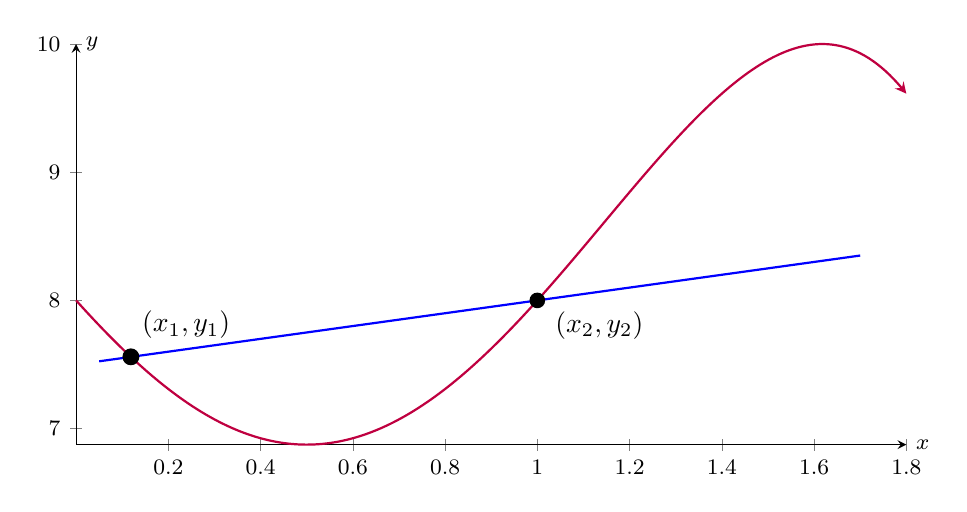
\begin{tikzpicture}
        \begin{axis}[
            my axis style,
            width=\textwidth,
            height=0.55\textwidth,
			ylabel = $y$,
			xlabel = $x$,
        ]
        
        \addplot[
            domain=0:1.8,
            thick,
            purple,
            ->
        ]
        {-2*x*x*x*x + 4*x*x*x + 2*x*x - 4*x + 8};

		\addplot[
            domain=0.05:1.7,
            thick,
            blue,
            -
        ]
        {0.5*x + 7.5};

  		\draw[fill=black] (0.1188,7.5599) circle(1mm);
		\node[label={80:{($x_1,y_1$)}},circle,fill,inner sep=2pt] at (0.1188,7.5599) {};
		\node[label={-10:{($x_2,y_2$)}},circle,fill,inner sep=2pt] at (1,8) {};
		%-2x^{4\ }+4x^{3}+2x^{2}-4x+1
    
        \fill[
            black
        ];
        
        \end{axis}
        \end{tikzpicture}
\end{center}

The slope of the secant line would be computed as,
$$m = \frac{y_2 - y_1}{x_2 - x_1}$$
If we replaced the $y-$coordinates with position vectors and the $x-$coordinates with time points, the slope of the secant line would represent the average velocity within the interval $[t_1,t_2]$.

\begin{thm}
Given a Pos v. Time graph of a moving body, the slope of a secant line in the interval $[t_1,t_2]$ represents the average velocity between $[t_1,t_2]$.
\end{thm}
\begin{pf}
	We proceed with similar reasoning from above, the slope of the secant line would be given as,
	$$m = \frac{\vec d_2 - \vec d_1}{t_2 - t_1} = \vec v_{av}$$
\end{pf}
\begin{defn}
A \textbf{tangent line} is a secant line, with the property that $x_2$ and $x_1$ are infinitesimally close apart.
\end{defn}
If $x_2$ and $x_1$ are infinitesimally close apart, then of course $y_2$ and $y_1$ must also be infinestesmly apart as well (How $y$ changes with respect to $x$ wouldn't matter at the infinitesimal level). As a result of this restriction, the tangent line to a graph would look as if it merely touches the graph at a single point, but in fact it does not, if we were to zoom in infinestesmly we would indeed observe that the tangent line touches the graph at two distinct points. Again it helps to provide an illustration,


\begin{center}
	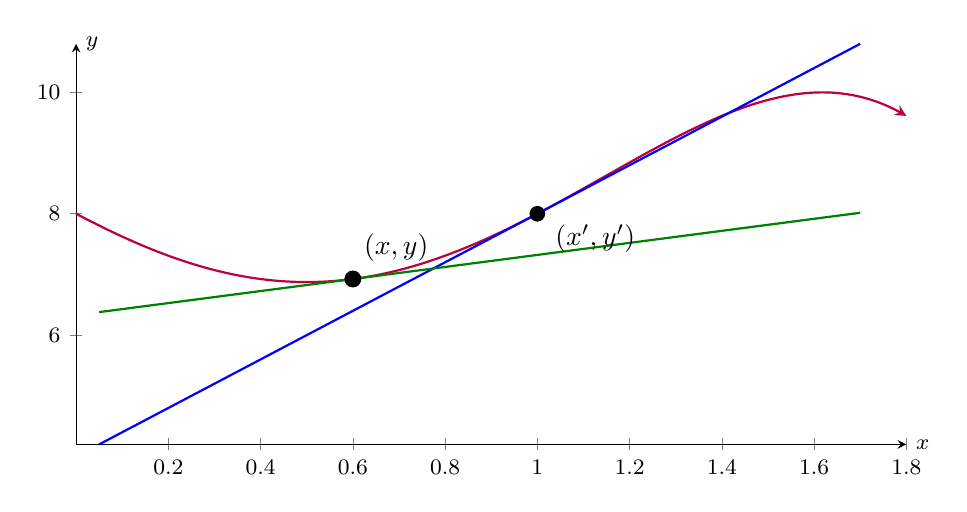
\begin{tikzpicture}
        \begin{axis}[
            my axis style,
            width=\textwidth,
            height=0.55\textwidth,
			ylabel = $y$,
			xlabel = $x$,
        ]
        
        \addplot[
            domain=0:1.8,
            thick,
            purple,
            ->
        ]
        {-2*x*x*x*x + 4*x*x*x + 2*x*x - 4*x + 8};

		\addplot[
            domain=0.05:1.7,
            thick,
            blue,
            -
        ]
        {4*x + 4};

		\addplot[
            domain=0.05:1.7,
            thick,
            Green,
            -
        ]
        {0.992*x + 6.3298};


  		\draw[fill=black] (0.6,6.925) circle(1mm);
		\node[label={80:{($x,y$)}},circle,fill,inner sep=2pt] at (0.6,6.925) {};
		\node[label={-10:{($x',y'$)}},circle,fill,inner sep=2pt] at (1,8) {};
		%-2x^{4\ }+4x^{3}+2x^{2}-4x+1
    
        \fill[
            black
        ];
        
        \end{axis}
        \end{tikzpicture}
\end{center}

This illustration provides \textbf{two} tangent lines, one at point $(x,y)$ and another at point $(x',y')$. Now if tangent lines are secant lines with property that the two intersected points are infinitesimally close apart, then we like to say that the $\emph{slope}$ of the tangent line provides us with the \textbf{exact} slope of the graph at any given point.

\begin{thm}
	Let the slope of a graph at some point $(x,y)$ be $m$. Let the tangent line to this graph at $(x,y)$ be $L$, then the slope of the tangent line $m_L = m$.
\end{thm}
\begin{pf}
At this stage, I am unable to prove this theorem as it would require knowledge of Calculus.
\end{pf}
At this point we can bridge the connection between the instantaneous velocity, $\vec v$ , and the idea of the tangent line. Since the slope of the tangent line provides us with the exact slope of the graph at a given point $(x,y)$, then we say that on a Pos v. Time graph, the slope of the tangent line at a given time $t$ provides us with the \emph{instantaneous} velocity. 
\begin{thm}
Given a Pos v. Time graph, let the tangent line at some point $(t, \vec d)$ be $L$. Then the slope of the tangent line $m_L$, is the instantaneous velocity $\vec v$ at time $t$.
\end{thm}
\begin{pf}
Again, at this stage, I am unable to prove this theorem as it would require knowledge of Calculus.
\end{pf}
\begin{ex}
Given the Pos v. Time graph below as well as a tangent line at time $t = 5$, compute the instantaneous velocity at time $t = 5$.
\begin{center}
	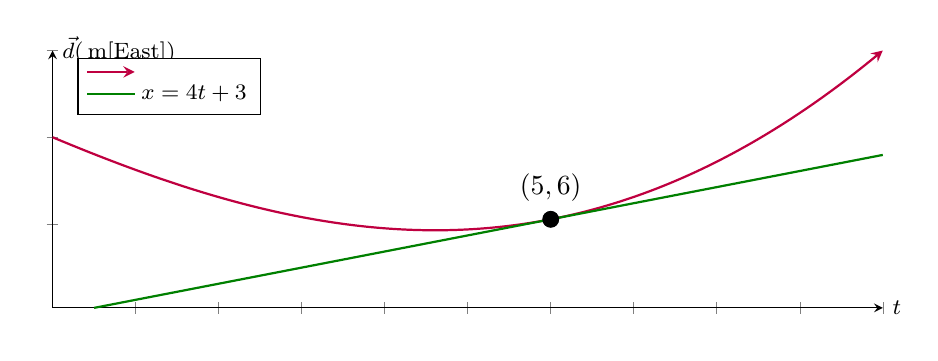
\begin{tikzpicture}
        \begin{axis}[
            my axis style,
            width=\textwidth,
            height=0.4\textwidth,
			ylabel = $\vec d (\m \tx{[East]})$,
			xlabel = $t$,
			yticklabels={,,},
			xticklabels={,,},
			legend entries={
					$ $,
					$x = 4t + 3$
				},
			legend pos=north west
        ]
        
        \addplot[
            domain=0:1,
            thick,
            purple,
            ->
        ]
        {-1*x*x*x*x + 4*x*x*x + 2*x*x - 4*x + 8};

		\addplot[
            domain=0.05:1,
            thick,
            Green,
            -
        ]
        {1.856*x + 5.9404};


  		\draw[fill=black] (0.6,7.054) circle(1mm);
		\node[label={90:{($5,6$)}},circle,fill,inner sep=2pt] at (0.6,7.054) {};
		%-2x^{4\ }+4x^{3}+2x^{2}-4x+1
    
        \fill[
            black
        ];
        
        \end{axis}
        \end{tikzpicture}
\end{center}
\end{ex}
\begin{soln}
$\implies$

\vspace*{4cm}
\end{soln}
\subsection{Extending concept to Acceleration}
Given a Pos v. Time plot, we have stated that the slope of the secant line over the interval $[t_1,t_2]$ gives us the average velocity over that time interval and that the slope of the tangent line at some time $t$ gives us the instantaneous velocity at that time $t$. However this concept can be extended over to acceleration as well, that is, if we are given the \emph{Velocity v. Time} plot, we can extract the average and instantaneous acceleration. We state their theorems below (Without proofs).
\begin{thm}
	Given a Velocity v. Time graph of a moving body, the slope of a secant line in the interval $[t_1,t_2]$ represents the average acceleration between $[t_1,t_2]$.
\end{thm}

\begin{thm}
	Given a Velocity v. Time graph, let the tangent line at some point $(t, \vec v)$ be $L$. Then the slope of the tangent line $m_L$, is the instantaneous acceleration $\vec a$ at time $t$.
\end{thm}

\begin{ex}
	Given the Velocity v. Time graph below as well as a tangent line at time $t = 5$, compute the instantaneous acceleration at time $t = 5$.
	\begin{center}
		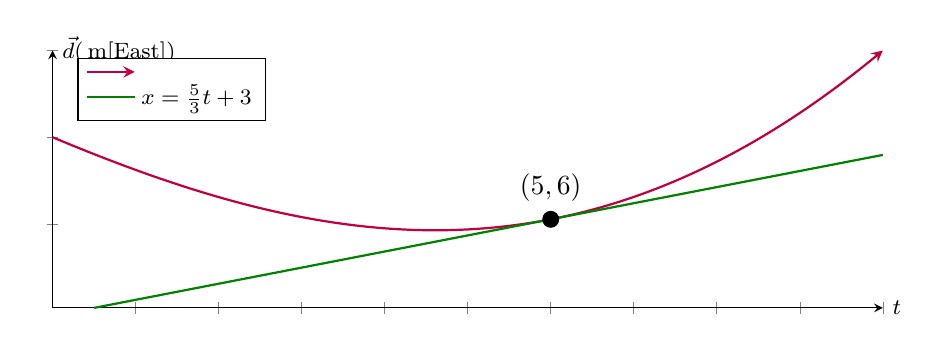
\begin{tikzpicture}
			\begin{axis}[
				my axis style,
				width=\textwidth,
				height=0.4\textwidth,
				ylabel = $\vec d (\m \tx{[East]})$,
				xlabel = $t$,
				yticklabels={,,},
				xticklabels={,,},
				legend entries={
						$ $,
						$x = \frac{5}{3}t + 3$
					},
				legend pos=north west
			]
			
			\addplot[
				domain=0:1,
				thick,
				purple,
				->
			]
			{-1*x*x*x*x + 4*x*x*x + 2*x*x - 4*x + 8};
	
			\addplot[
				domain=0.05:1,
				thick,
				Green,
				-
			]
			{1.856*x + 5.9404};
	
	
			  \draw[fill=black] (0.6,7.054) circle(1mm);
			\node[label={90:{($5,6$)}},circle,fill,inner sep=2pt] at (0.6,7.054) {};
			%-2x^{4\ }+4x^{3}+2x^{2}-4x+1
		
			\fill[
				black
			];
			
			\end{axis}
			\end{tikzpicture}
	\end{center}
	\end{ex}
	\begin{soln}
	$\implies$
	
	\vspace*{4cm}
\end{soln}
\begin{ex}
A horse had a forward velocity of $\vec v_i = 500 \m / \s \tx{[East]}$ and then began to accelerate at an average acceleration of $\vec a_{av} = 54 \m / \s^2 \tx{[West]}$ over a duration of $\Delta t = 24 \s$. Compute his final velocity.
\end{ex}
\begin{soln}
$\implies$
\vspace*{5cm}
\end{soln}

	
\subsection{Non-Linear Position v. Time plots}
\begin{enumerate}[label = (\alph*)]
	\item 
        \begin{tikzpicture}
        \begin{axis}[
            my axis style,
            width=\textwidth,
            height=.5\textwidth,
			ylabel = $\vec d (\tx{m [East]})$,
			xlabel = $t$,
        ]
        
        \addplot[
            domain=0:5,
            thick,
            purple,
            ->
        ]
        {x*x};
    
        \fill[
            black
        ];
        
        \end{axis}
        \end{tikzpicture}

		\textbf{\large{Properties of type (a):}}
		\begin{itemize}
			\item The object is experiencing \textbf{non-uniform motion}.
			\item The object is \textbf{speeding up}
			\item The object is moving [East] relative to the reference point (0,0).
		\end{itemize}


	\item 
	\begin{tikzpicture}
        \begin{axis}[
            my axis style,
            width=\textwidth,
            height=.5\textwidth,
			ylabel = $ $,
			xlabel = $t$,
        ]
        
        \addplot[
            domain=0:5,
            thick,
            purple,
            ->
        ]
        {-1*x*x};
    
        \fill[
            black
        ];
        
        \end{axis}
        \end{tikzpicture}

		\textbf{\large{Properties of type (b):}}
		\begin{itemize}
			\item The object is experiencing \textbf{non-uniform motion}.
			\item The object is \textbf{speeding up}
			\item The object is moving [West] relative to the reference point (0,0).
		\end{itemize}


	\item 
	\begin{tikzpicture}
        \begin{axis}[
            my axis style,
            width=\textwidth,
            height=.5\textwidth,
			ylabel = $\vec d (\tx{m [East]})$,
			xlabel = $t$,
        ]
        
        \addplot[
            domain=0:2.2,
            thick,
            purple,
            ->
        ]
        {-1*x*x + 4*x};
    
        \fill[
            black
        ];
        
        \end{axis}
        \end{tikzpicture}

		\textbf{\large{Properties of type (c):}}
		\begin{itemize}
			\item The object is experiencing \textbf{non-uniform motion}.
			\item The object is \textbf{slowing down}
			\item The object is moving [East] relative to the reference point (0,0).
		\end{itemize}

	\item 
	\begin{tikzpicture}
        \begin{axis}[
            my axis style,
            width=\textwidth,
            height=.5\textwidth,
			ylabel = $ $,
			xlabel = $t$,
        ]
        
        \addplot[
            domain=0:2.2,
            thick,
            purple,
            ->
        ]
        {x*x - 4*x};
    
        \fill[
            black
        ];
        
        \end{axis}
        \end{tikzpicture}

		\textbf{\large{Properties of type (d):}}
		\begin{itemize}
			\item The object is experiencing \textbf{non-uniform motion}.
			\item The object is \textbf{slowing down}
			\item The object is moving [West] relative to the reference point (0,0).
		\end{itemize}

\end{enumerate}

\newpage
\subsection{Going from Velocity to displacement}




	


\end{document}
